% =============================================================================
% PCIe 7.0 Controller IP — Technical Specification
% =============================================================================
\documentclass[11pt,a4paper]{article}

% --- Packages ----------------------------------------------------------------
\usepackage[top=25mm,bottom=25mm,left=25mm,right=25mm]{geometry}
\usepackage[T1]{fontenc}
\usepackage[utf8]{inputenc}
\usepackage{lmodern}
\usepackage{microtype}
\usepackage{hyperref}
\usepackage{xcolor}
\usepackage{booktabs}
\usepackage{longtable}
\usepackage{array}
\usepackage{multirow}
\usepackage{tabularx}
\usepackage{graphicx}
\usepackage{tikz}
\usetikzlibrary{arrows.meta,positioning,shapes.geometric,fit,backgrounds,calc}
\usepackage{listings}
\usepackage{fancyhdr}
\usepackage{titlesec}
\usepackage{tocloft}
\usepackage{amsmath}
\usepackage{amssymb}
\usepackage{pifont}
\usepackage{enumitem}
\usepackage{mdframed}
\usepackage{colortbl}
\usepackage{caption}
\usepackage{subcaption}

% --- Colors ------------------------------------------------------------------
\definecolor{scblue}{RGB}{0,70,140}
\definecolor{scgray}{RGB}{90,90,90}
\definecolor{scgreen}{RGB}{0,120,60}
\definecolor{scorange}{RGB}{210,90,0}
\definecolor{lightgray}{RGB}{240,240,240}
\definecolor{tablehead}{RGB}{0,70,140}

% --- Hyperref setup ----------------------------------------------------------
\hypersetup{
  colorlinks=true,
  linkcolor=scblue,
  urlcolor=scblue,
  citecolor=scgreen,
  pdftitle={PCIe 7.0 Controller -- Technical Specification},
  pdfauthor={SiliconCraft},
  pdfsubject={PCIe 7.0 IP Core Specification},
}

% --- Page style --------------------------------------------------------------
\pagestyle{fancy}
\fancyhf{}
\fancyhead[L]{\small\textcolor{scgray}{PCIe 7.0 Controller IP}}
\fancyhead[R]{\small\textcolor{scgray}{Technical Specification v0.2.0}}
\fancyfoot[C]{\small\textcolor{scgray}{\thepage}}
\fancyfoot[L]{\small\textcolor{scgray}{CONFIDENTIAL --- SiliconCraft}}
\fancyfoot[R]{\small\textcolor{scgray}{2026-05-21}}
\renewcommand{\headrulewidth}{0.4pt}
\renewcommand{\footrulewidth}{0.4pt}

% --- Section formatting ------------------------------------------------------
\titleformat{\section}{\large\bfseries\color{scblue}}{}{0em}{\thesection\quad}
\titleformat{\subsection}{\normalsize\bfseries\color{scblue}}{}{0em}{\thesubsection\quad}
\titleformat{\subsubsection}{\normalsize\bfseries\color{scgray}}{}{0em}{\thesubsubsection\quad}

% --- Code listings -----------------------------------------------------------
\lstset{
  basicstyle=\small\ttfamily,
  keywordstyle=\bfseries\color{scblue},
  commentstyle=\itshape\color{scgray},
  stringstyle=\color{scgreen},
  breaklines=true,
  frame=single,
  rulecolor=\color{scgray},
  backgroundcolor=\color{lightgray},
  numbers=left,
  numberstyle=\tiny\color{scgray},
  tabsize=2,
}

% --- Table header macro ------------------------------------------------------
\newcommand{\theadcell}[1]{%
  \cellcolor{tablehead}\textcolor{white}{\textbf{#1}}}

% --- Note box ----------------------------------------------------------------
\newmdenv[
  backgroundcolor=lightgray,
  linecolor=scblue,
  linewidth=1pt,
  innerleftmargin=8pt,
  innerrightmargin=8pt,
  innertopmargin=6pt,
  innerbottommargin=6pt,
]{notebox}

% =============================================================================
\begin{document}

% --- Title Page --------------------------------------------------------------
\begin{titlepage}
  \begin{tikzpicture}[remember picture, overlay]
    \fill[scblue] (current page.north west) rectangle
      ([yshift=-60mm]current page.north east);
    \fill[scgray!20] (current page.south west) rectangle
      ([yshift=20mm]current page.south east);
  \end{tikzpicture}

  \vspace*{20mm}
  {\color{white}\fontsize{28}{34}\selectfont\bfseries PCIe 7.0 Controller IP}\\[4mm]
  {\color{white!80!scblue}\fontsize{16}{20}\selectfont Technical Specification}

  \vspace{40mm}

  \begin{tabular}{ll}
    \textbf{Document number} & SC-PCIE7-SPEC-001 \\[2mm]
    \textbf{Version}         & 0.2.0 \\[2mm]
    \textbf{Date}            & 2026-05-21 \\[2mm]
    \textbf{Status}          & Engineering Release \\[2mm]
    \textbf{Author}          & SiliconCraft Design Team \\[2mm]
    \textbf{Top module}      & \texttt{pcie\_controller\_top} \\[2mm]
    \textbf{Technology}      & Process-independent RTL \\[2mm]
    \textbf{Classification}  & Confidential \\
  \end{tabular}

  \vfill

  \begin{notebox}
    \textbf{Note:} This document describes the \texttt{pcie\_controller\_top} IP as
    an engineering deliverable. It is not a PCI-SIG compliance certification.
    All compliance claims are limited to the evidence in \texttt{docs/compliance\_matrix.md}.
  \end{notebox}
\end{titlepage}

% --- Revision History --------------------------------------------------------
\newpage
\section*{Revision History}
\begin{tabular}{llll}
  \toprule
  \theadcell{Version} & \theadcell{Date} & \theadcell{Author} & \theadcell{Changes} \\
  \midrule
  0.1.0 & 2026-05-17 & Design Team & Initial commit: full RTL stack, 10-test directed TB \\
  0.2.0 & 2026-05-21 & Design Team & Added: SVA suites, UVM PIPE agent, error injection,
                                     PM RTL, CDC sync, completion timeout, UPF, formal,
                                     IP-XACT, integration guide, synthesis script \\
  0.2.1 & 2026-05-21 & Design Team & Refined: DLL activation SM, 3-phase EQ, DLCRC-16,
                                     FC credit return, delivery assertions expanded,
                                     extended register map, PIPE signal detail \\
  \bottomrule
\end{tabular}

\tableofcontents
\newpage

% =============================================================================
\section{Introduction}
% =============================================================================

\subsection{Purpose}

This specification defines the functional and interface contract for the
\texttt{pcie\_controller\_top} PCIe~7.0 Controller IP. It covers:

\begin{itemize}[noitemsep]
  \item Feature set and parameterization
  \item Port list and interface definitions
  \item Protocol layer descriptions (Physical, Data Link, Transaction)
  \item Link equalization (Gen3+) protocol
  \item Configuration space register map (standard + AER extended)
  \item Power management architecture
  \item Clock domain and reset structure
  \item Verification and delivery collateral
\end{itemize}

\subsection{Scope and Limitations}

This IP is a simulation-verified RTL model for educational, portfolio, and
prototype integration use. The following are \textbf{outside scope}:

\begin{itemize}[noitemsep]
  \item PCI-SIG compliance certification or logo program qualification
  \item PHY electrical layer (represented by PIPE-level BFM)
  \item FLIT-mode framing (planned for v0.3.0)
  \item Ordering rule enforcement (planned for v0.3.0)
\end{itemize}

\subsection{Referenced Documents}

\begin{tabular}{ll}
  \toprule
  \theadcell{Reference} & \theadcell{Document} \\
  \midrule
  {[}PCI-SIG-7{]}  & PCI Express Base Specification, Revision~7.0 \\
  {[}PIPE-6{]}     & PCI Express PHY Interface for the PCI Express Architecture, v6.0 \\
  {[}AXI-AMBA{]}   & AMBA AXI and ACE Protocol Specification, v2.0 \\
  {[}IEEE-1801{]}  & IEEE Standard for Design and Verification of Low-Power, Energy-Aware Electronic Systems (UPF) \\
  {[}IEEE-1685{]}  & IEEE Standard for IP-XACT \\
  {[}IEEE-1800{]}  & IEEE Standard for SystemVerilog \\
  \bottomrule
\end{tabular}

% =============================================================================
\section{Feature Overview}
% =============================================================================

\subsection{Key Features}

\begin{tabular}{p{5cm}p{9cm}}
  \toprule
  \theadcell{Feature} & \theadcell{Description} \\
  \midrule
  PCIe Generation & Gen1 (2.5\,GT/s) through Gen7 (128\,GT/s), parameterized \\
  Lane Width       & $\times$1, $\times$2, $\times$4, $\times$8, $\times$16 \\
  Device Role      & Endpoint (EP), Root Port (RP), Dual Mode (DM), Switch Port (SW) \\
  AXI Interface    & AXI4 Subordinate (inbound) + AXI4 Manager (completions), 256-bit \\
  DMA Engine       & 4-channel H2D/D2H, MRRS/MPS-bounded chunking, 256-tag pool \\
  MSI / MSI-X      & Up to 32 MSI vectors; up to 2048 MSI-X vectors \\
  AER              & Advanced Error Reporting: correctable, non-fatal, fatal \\
  Flow Control     & Credit-based FC: Posted, Non-Posted, Completion (infinite support) \\
  DLL              & 12-bit sequence numbers, LCRC-32, 4096-entry replay buffer; DLCRC-16 on DLLPs \\
  DLL Activation   & State machine: DL\_INACTIVE $\to$ DL\_INIT $\to$ DL\_ACTIVE $\to$ DL\_ERROR \\
  LTSSM            & Full 28-state machine per PCIe~7.0 \S4.2 with 3-phase equalization \\
  Equalization     & Gen3+ 4-phase EQ: Phase0 (preset), Phase1 (2\,ms), Phase2 (2\,ms), Phase3 (50\,$\mu$s) \\
  Power Management & L0s auto-entry (EIOS-based), L1 DLLP handshake, L2 software entry, PME wake \\
  Completion Timeout & Per-tag countdown timers, Range B default (50\,ms), correctable error \\
  CDC Synchronizers & 2-flop sync, pulse sync, reset sync, async FIFO (Gray-code) \\
  Config Space     & 4\,KB Type-0/Type-1, PCIe Cap, PM Cap, MSI, MSI-X, AER \\
  \bottomrule
\end{tabular}

\subsection{Top-Level Parameters}

\begin{tabular}{lllp{6cm}}
  \toprule
  \theadcell{Parameter} & \theadcell{Type} & \theadcell{Default} & \theadcell{Description} \\
  \midrule
  \texttt{DEVICE\_ROLE}   & \texttt{pcie\_role\_e} & \texttt{ROLE\_EP}   & EP / RP / DM / SW \\
  \texttt{MAX\_GEN}       & \texttt{pcie\_gen\_e}  & \texttt{PCIE\_GEN7} & Maximum PCIe generation \\
  \texttt{NUM\_LANES}     & \texttt{int}           & 16                  & $\times$1 to $\times$16 \\
  \texttt{DATA\_W}        & \texttt{int}           & 256                 & Internal / AXI data width (bits) \\
  \texttt{ADDR\_W}        & \texttt{int}           & 64                  & AXI address width (bits) \\
  \texttt{AXI\_ID\_W}     & \texttt{int}           & 8                   & AXI ID width (bits) \\
  \texttt{PIPE\_W}        & \texttt{int}           & 32                  & PIPE data width per lane (bits) \\
  \texttt{VENDOR\_ID}     & \texttt{logic[15:0]}   & \texttt{16'hCAFE}   & PCIe Vendor ID \\
  \texttt{DEVICE\_ID}     & \texttt{logic[15:0]}   & \texttt{16'h0001}   & PCIe Device ID \\
  \texttt{BAR0\_APERTURE} & \texttt{logic[7:0]}    & 24                  & BAR0 size: $2^n$ bytes \\
  \texttt{EN\_MSI}        & \texttt{bit}           & 1                   & Enable MSI capability \\
  \texttt{EN\_MSIX}       & \texttt{bit}           & 1                   & Enable MSI-X capability \\
  \texttt{EN\_AER}        & \texttt{bit}           & 1                   & Enable AER extended capability \\
  \texttt{EN\_ECRC}       & \texttt{bit}           & 1                   & Enable ECRC generation/checking \\
  \texttt{EN\_DMA}        & \texttt{bit}           & 1                   & Enable DMA engine \\
  \texttt{DMA\_CHANNELS}  & \texttt{int}           & 4                   & Concurrent DMA channels \\
  \bottomrule
\end{tabular}

% =============================================================================
\section{Architecture}
% =============================================================================

\subsection{Block Diagram}

Figure~\ref{fig:blockdiag} shows the top-level functional block diagram.

\begin{figure}[h!]
\centering
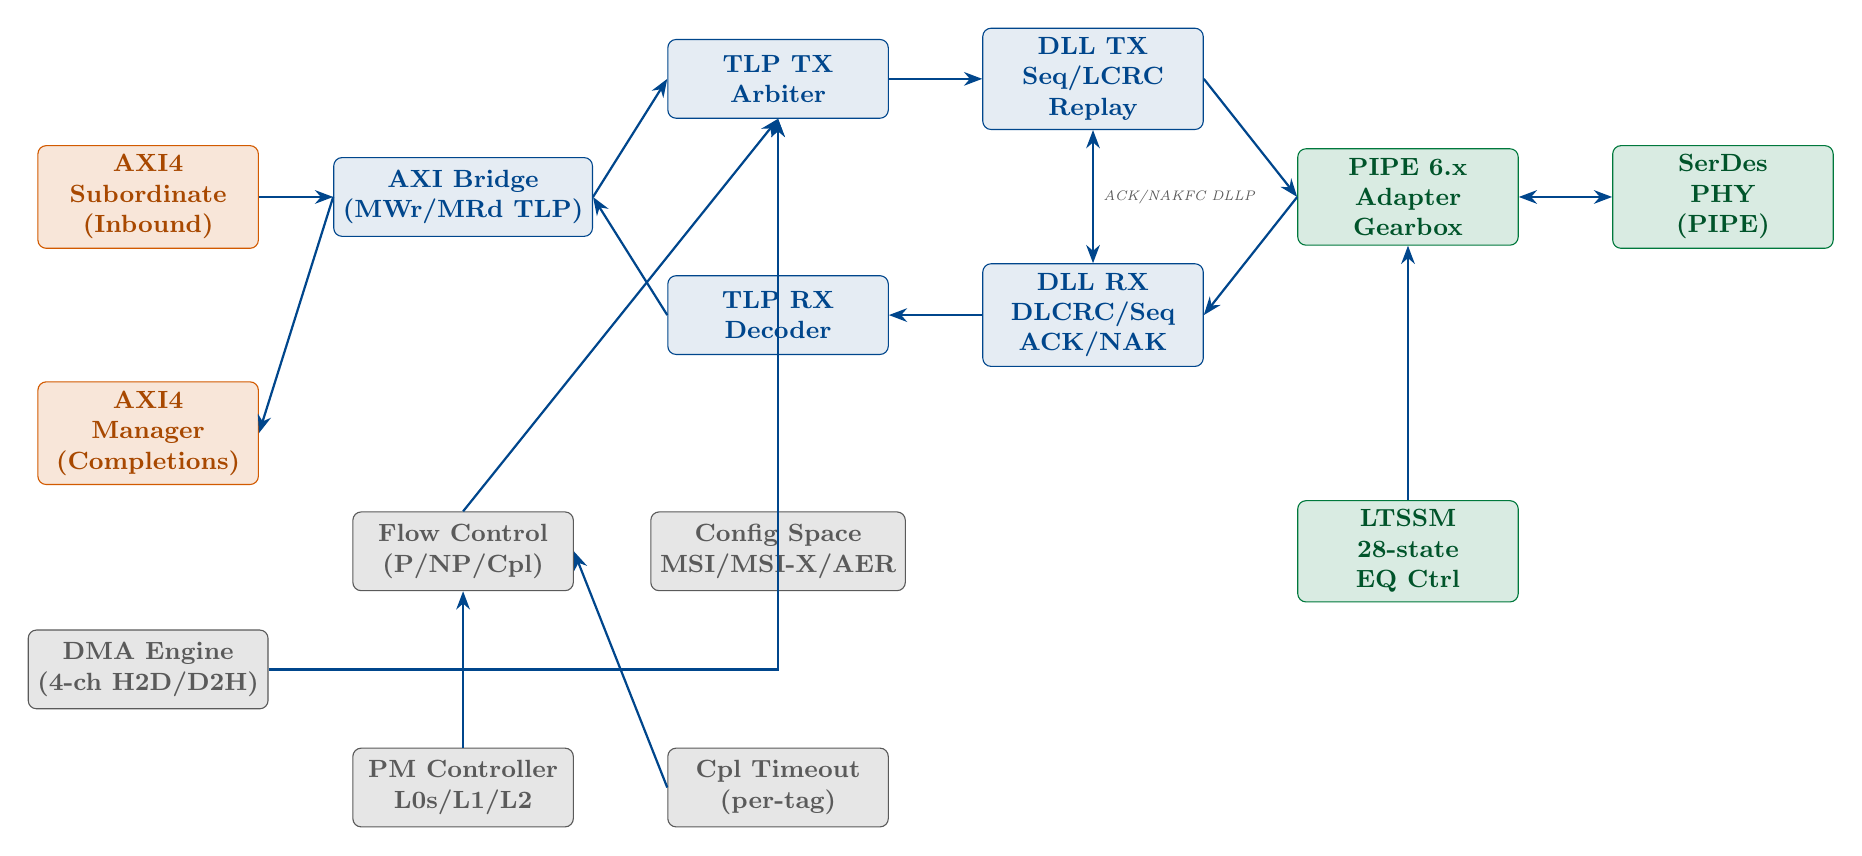
\begin{tikzpicture}[
  box/.style={draw=scblue, fill=scblue!10, rounded corners=3pt,
              minimum width=28mm, minimum height=10mm, font=\small\bfseries,
              align=center, text=scblue},
  phy/.style={box, fill=scgreen!15, draw=scgreen, text=scgreen!70!black},
  app/.style={box, fill=scorange!15, draw=scorange, text=scorange!80!black},
  mgmt/.style={box, fill=scgray!15, draw=scgray, text=scgray},
  arr/.style={-Stealth, thick, color=scblue},
  darr/.style={Stealth-Stealth, thick, color=scblue},
  label/.style={font=\tiny\itshape, color=scgray},
  >=Stealth
]

% Application layer
\node[app] (axi_sub) at (0,0)    {AXI4\\Subordinate\\(Inbound)};
\node[app] (axi_mgr) at (0,-3)   {AXI4\\Manager\\(Completions)};
\node[mgmt] (dma)    at (0,-6)   {DMA Engine\\(4-ch H2D/D2H)};

% AXI Bridge
\node[box] (bridge)  at (4,0)    {AXI Bridge\\(MWr/MRd TLP)};

% Transaction layer
\node[box] (tlp_tx)  at (8,1.5)  {TLP TX\\Arbiter};
\node[box] (tlp_rx)  at (8,-1.5) {TLP RX\\Decoder};
\node[mgmt] (cfg)    at (8,-4.5) {Config Space\\MSI/MSI-X/AER};
\node[mgmt] (fc)     at (4,-4.5) {Flow Control\\(P/NP/Cpl)};

% Data Link layer
\node[box] (dll_tx)  at (12,1.5) {DLL TX\\Seq/LCRC\\Replay};
\node[box] (dll_rx)  at (12,-1.5){DLL RX\\DLCRC/Seq\\ACK/NAK};

% Physical layer
\node[phy] (pipe)    at (16,0)   {PIPE 6.x\\Adapter\\Gearbox};
\node[phy] (ltssm)   at (16,-4.5){LTSSM\\28-state\\EQ Ctrl};

% PHY
\node[phy] (phy)     at (20,0)   {SerDes\\PHY\\(PIPE)};

% New RTL blocks
\node[mgmt] (pm)     at (4,-7.5) {PM Controller\\L0s/L1/L2};
\node[mgmt] (cplto)  at (8,-7.5) {Cpl Timeout\\(per-tag)};

% Connections --- application
\draw[arr] (axi_sub.east) -- (bridge.west);
\draw[arr] (bridge.west)  -- (axi_mgr.east);
\draw[arr] (dma.east)     -| (tlp_tx.south);

% Connections --- TL
\draw[arr] (bridge.east)  -- (tlp_tx.west);
\draw[arr] (tlp_rx.west)  -- (bridge.east);
\draw[arr] (fc.north)     -- (tlp_tx.south);
\draw[arr] (cfg.north)    -- (tlp_tx.south);

% Connections --- DLL
\draw[arr] (tlp_tx.east)  -- (dll_tx.west);
\draw[arr] (dll_rx.west)  -- (tlp_rx.east);
\draw[darr] (dll_tx.south) -- (dll_rx.north) node[label,midway,right]{ACK/NAK\\FC DLLP};

% Connections --- PIPE
\draw[arr] (dll_tx.east)  -- (pipe.west);
\draw[arr] (pipe.west)    -- (dll_rx.east);
\draw[arr] (ltssm.north)  -- (pipe.south);

% Connections --- PHY
\draw[darr] (pipe.east) -- (phy.west);

% PM and cpl timeout
\draw[arr] (pm.north)  -- (fc.south);
\draw[arr] (cplto.west) -- (fc.east);

\end{tikzpicture}
\caption{PCIe 7.0 Controller --- Top-Level Functional Block Diagram}
\label{fig:blockdiag}
\end{figure}

\subsection{Layer Responsibilities}

\begin{description}[leftmargin=3cm, style=nextline]
  \item[Physical Layer] LTSSM manages the 28-state link training machine with
    full 3-phase equalization support (Gen3+). The PIPE~6.x adapter implements
    the TX gearbox (256-bit $\to$ $N\times$PIPE\_W), K-symbol insertion
    (STP/SDP/END\_/EDB), and RX assembly. CDC synchronizers
    (\texttt{pcie\_cdc\_sync.sv}) and async FIFOs
    (\texttt{pcie\_async\_fifo.sv}) handle the \texttt{core\_clk}/\texttt{pipe\_clk}
    crossing. L0S is entered on EIOS reception; L1 requires PM DLLP handshake.

  \item[Data Link Layer] TX assigns 12-bit sequence numbers and appends CRC-32 LCRC.
    A 4096-entry replay buffer holds outstanding TLPs. RX validates sequence and CRC,
    generates ACK/NAK DLLPs, and decodes incoming DLLPs (FC~Init, FC~Update, PM).
    All DLLPs are protected with DLCRC-16 (polynomial 0x8005). The DLL activation
    state machine (DL\_INACTIVE $\to$ DL\_INIT $\to$ DL\_ACTIVE $\to$ DL\_ERROR)
    controls \texttt{dll\_link\_active} and enforces a replay count limit of 3
    before asserting \texttt{dll\_error}.

  \item[Transaction Layer] TX arbiter round-robins four input ports (AXI bridge Posted,
    AXI bridge Non-Posted, DMA, Config Space), gated by Flow Control credits.
    RX decodes the 3DW/4DW header, routes to the appropriate sink (AXI bridge,
    config space, DMA, completion buffer), and reports poisoned/malformed TLP errors.

  \item[AXI Bridge] Maps AXI4 write transactions to Memory Write TLPs (MWr32/MWr64)
    and AXI4 read transactions to Memory Read TLPs (MRd32/MRd64), with a 256-entry
    tag pool for outstanding reads. Returning CplD are reassembled into AXI R-channel
    responses.

  \item[DMA Engine] Issues host-to-device MRd64 TLPs (MRRS-bounded), assembles
    completions, and writes to local AXI memory. Device-to-host issues MWr64 TLPs
    (MPS-bounded). Uses tag range 512--767, reserving 0--511 for AXI bridge.

  \item[Config Space] Implements a 4\,KB Type-0/Type-1 configuration space with
    capabilities at fixed offsets: PCIe Cap (0x40), PM Cap (0x80), MSI Cap (0x90),
    MSI-X Cap (0xA0, 2048 vectors), AER Extended Cap (0x100). RW1C error registers.

  \item[Power Management] \texttt{pcie\_pm\_ctrl} FSM handles L0s auto-entry on idle
    (triggered by EIOS detection), L1 DLLP handshake (PM\_Enter\_L1 / PM\_Req\_Ack),
    software-initiated L2, and PME wakeup. Drives DLLP requests to DLL TX and
    LTSSM power-state requests.

  \item[Completion Timeout] \texttt{pcie\_cpl\_timeout} maintains per-tag countdown
    timers. On expiry (default Range~B, 50\,ms), pulses \texttt{cfg\_err\_cor} and
    reports the offending tag.
\end{description}

% =============================================================================
\section{Port List}
% =============================================================================

\subsection{Clock and Reset}

\begin{tabular}{lllp{7cm}}
  \toprule
  \theadcell{Port} & \theadcell{Dir} & \theadcell{Width} & \theadcell{Description} \\
  \midrule
  \texttt{core\_clk}   & in  & 1 & Core / application clock \\
  \texttt{core\_rst\_n}& in  & 1 & Active-low async reset; deassert synchronous to \texttt{core\_clk} via \texttt{pcie\_rst\_sync} \\
  \texttt{pipe\_clk}   & in  & 1 & PIPE reference clock from PHY \\
  \texttt{aux\_clk}    & in  & 1 & Always-on auxiliary clock for power management \\
  \bottomrule
\end{tabular}

\subsection{PIPE Interface}

\begin{tabular}{lllp{7.5cm}}
  \toprule
  \theadcell{Port} & \theadcell{Dir} & \theadcell{Width} & \theadcell{Description} \\
  \midrule
  \texttt{pipe\_tx\_data}       & out & $N\times$PIPE\_W & TX data (per lane) \\
  \texttt{pipe\_tx\_datak}      & out & $N\times$PIPE\_W/8 & TX K-symbol indicator \\
  \texttt{pipe\_tx\_elec\_idle} & out & $N$ & Electrical idle request \\
  \texttt{pipe\_tx\_compliance} & out & $N$ & Compliance pattern enable \\
  \texttt{pipe\_tx\_deemph}     & out & $N$ & TX de-emphasis select \\
  \texttt{pipe\_tx\_margin}     & out & $N\times 3$ & TX margin control \\
  \texttt{pipe\_tx\_swing}      & out & $N$ & TX voltage swing \\
  \texttt{pipe\_tx\_eq\_ctrl}   & out & $N\times 2$ & Equalization preset \\
  \texttt{pipe\_rx\_data}       & in  & $N\times$PIPE\_W & RX data (per lane); valid when \texttt{pipe\_rx\_valid} \\
  \texttt{pipe\_rx\_datak}      & in  & $N\times$PIPE\_W/8 & RX K-symbol indicator; set for COM, PAD, IDLE \\
  \texttt{pipe\_rx\_valid}      & in  & $N$ & RX data valid; qualified by \texttt{pipe\_rx\_status} \\
  \texttt{pipe\_rx\_elec\_idle} & in  & $N$ & Electrical idle detect from PHY (EIOS trigger) \\
  \texttt{pipe\_rx\_status\_valid} & in & $N$ & RX status valid; qualifies \texttt{pipe\_rx\_status} \\
  \texttt{pipe\_rx\_status}     & in  & $N\times 3$ & RX status code (see Table~\ref{tab:rxstatus}) \\
  \texttt{pipe\_power\_down}    & out & 4 & Power-down mode (see Table~\ref{tab:powerdown}) \\
  \texttt{pipe\_reset\_n}       & out & 1 & PIPE reset (active-low); deasserted when LTSSM exits DETECT \\
  \texttt{pipe\_rate}           & out & 4 & Speed select (see Table~\ref{tab:piperate}) \\
  \texttt{pipe\_width}          & out & 2 & Lane width select: 00=$\times$1, 01=$\times$2, 10=$\times$4, 11=$\times$8+ \\
  \texttt{pipe\_clk\_req\_n}    & in  & 1 & Clock request (active-low); used for L1 gating \\
  \bottomrule
\end{tabular}

\noindent $N$ = \texttt{NUM\_LANES} parameter.

\vspace{4mm}

\noindent\textbf{Table~\ref{tab:rxstatus}: \texttt{pipe\_rx\_status[2:0]} Encoding}
\begin{table}[h!]
\label{tab:rxstatus}
\centering
\begin{tabular}{llp{9cm}}
  \toprule
  \theadcell{Code} & \theadcell{Name} & \theadcell{Description} \\
  \midrule
  3'b000 & IDLE         & No special status; normal operation \\
  3'b001 & RECV\_DET    & Receiver detected (used in DETECT state); also TS1 symbol-lock in POLLING \\
  3'b010 & EIOS\_TS2    & EIOS (Electrical Idle Ordered Set) received or TS2 detected in POLLING \\
  3'b011 & TS\_LOCK     & TS1/TS2 ordered-set lock achieved \\
  3'b100 & SPEED\_CHG   & Speed change request in progress (rate change underway) \\
  3'b101 & PHYSTATUS    & PHY status event (assert-pulse semantics from PIPE spec) \\
  3'b110 & RSVD         & Reserved \\
  3'b111 & RSVD         & Reserved \\
  \bottomrule
\end{tabular}
\caption{\texttt{pipe\_rx\_status[2:0]} code definitions per PIPE~6.x}
\end{table}

\noindent\textbf{Table~\ref{tab:piperate}: \texttt{pipe\_rate[3:0]} Encoding}
\begin{table}[h!]
\label{tab:piperate}
\centering
\begin{tabular}{lll}
  \toprule
  \theadcell{Code} & \theadcell{Speed} & \theadcell{Generation} \\
  \midrule
  4'b0001 & 2.5\,GT/s  & Gen 1 \\
  4'b0010 & 5.0\,GT/s  & Gen 2 \\
  4'b0011 & 8.0\,GT/s  & Gen 3 (128b/130b) \\
  4'b0100 & 16.0\,GT/s & Gen 4 \\
  4'b0101 & 32.0\,GT/s & Gen 5 \\
  4'b0110 & 64.0\,GT/s & Gen 6 (FLIT/NRZ) \\
  4'b0111 & 128.0\,GT/s& Gen 7 (FLIT/PAM4) \\
  \bottomrule
\end{tabular}
\caption{\texttt{pipe\_rate[3:0]} speed select encoding}
\end{table}

\noindent\textbf{Table~\ref{tab:powerdown}: \texttt{pipe\_power\_down[3:0]} Encoding}
\begin{table}[h!]
\label{tab:powerdown}
\centering
\begin{tabular}{lllp{7cm}}
  \toprule
  \theadcell{Code} & \theadcell{State} & \theadcell{LTSSM Use} & \theadcell{Description} \\
  \midrule
  4'b0000 & P0   & L0, L0s, Equalization & Full power; TX and RX active \\
  4'b0001 & P0s  & L0s TX, Recovery entry & Low-power TX idle; RX maintained \\
  4'b0010 & P1   & L1 entry/idle & Both TX and RX clocks stopped; retains CDR lock \\
  4'b0100 & P2   & L2 idle        & Deepest power state; CDR lock lost; requires full re-training \\
  \bottomrule
\end{tabular}
\caption{\texttt{pipe\_power\_down[3:0]} power-state encoding}
\end{table}

\subsection{AXI4 Subordinate Interface}

All signals prefixed \texttt{s\_axi\_}; standard AXI4 write and read channels.
Data width = DATA\_W, address width = ADDR\_W, ID width = AXI\_ID\_W.
\texttt{AWBURST} and \texttt{ARBURST} must be \texttt{INCR} (2'b01).

\subsection{AXI4 Manager Interface}

All signals prefixed \texttt{m\_axi\_}; driven by PCIe completions toward system memory.
Same widths as subordinate interface.

\subsection{DMA Interface}

\begin{tabular}{lllp{7.5cm}}
  \toprule
  \theadcell{Port} & \theadcell{Dir} & \theadcell{Width} & \theadcell{Description} \\
  \midrule
  \texttt{dma\_start}    & in  & 1  & One-cycle pulse: start DMA transfer \\
  \texttt{dma\_src\_addr}& in  & 64 & Source address (host or device) \\
  \texttt{dma\_dst\_addr}& in  & 64 & Destination address \\
  \texttt{dma\_length}   & in  & 32 & Transfer length in bytes \\
  \texttt{dma\_dir}      & in  & 1  & Direction: 0 = H2D, 1 = D2H \\
  \texttt{dma\_done}     & out & 1  & One-cycle pulse: transfer complete \\
  \texttt{dma\_error}    & out & 1  & One-cycle pulse: transfer error \\
  \bottomrule
\end{tabular}

\subsection{Interrupt Interface}

\begin{tabular}{lllp{7.5cm}}
  \toprule
  \theadcell{Port} & \theadcell{Dir} & \theadcell{Width} & \theadcell{Description} \\
  \midrule
  \texttt{msi\_irq}     & out & 1  & MSI interrupt pulse \\
  \texttt{msi\_vector}  & out & 5  & MSI vector index (0--31) \\
  \texttt{msix\_irq}    & out & 1  & MSI-X interrupt pulse \\
  \texttt{msix\_vector} & out & 11 & MSI-X vector index (0--2047) \\
  \texttt{intx\_assert} & in  & 1  & Legacy INTx assertion request \\
  \bottomrule
\end{tabular}

\subsection{Status and Debug}

\begin{tabular}{lllp{7.5cm}}
  \toprule
  \theadcell{Port} & \theadcell{Dir} & \theadcell{Width} & \theadcell{Description} \\
  \midrule
  \texttt{link\_up}           & out & 1 & Link in L0 state \\
  \texttt{ltssm\_state}       & out & 6 & Current LTSSM state (6-bit \texttt{ltssm\_state\_e}) \\
  \texttt{ltssm\_status}      & out & 32 & LTSSM status register (negotiated gen/width, EQ phase, DLL active) \\
  \texttt{dll\_link\_active}  & out & 1 & DLL layer operational; FC Init complete and DL\_ACTIVE reached \\
  \texttt{eq\_phase}          & out & 3 & Current equalization phase (0--3, Gen3+ only) \\
  \texttt{negotiated\_gen}    & out & 4 & Negotiated PCIe generation \\
  \texttt{negotiated\_width}  & out & 5 & Negotiated lane width \\
  \texttt{cfg\_err\_cor}      & out & 1 & Correctable error detected \\
  \texttt{cfg\_err\_nonfatal} & out & 1 & Non-fatal uncorrectable error \\
  \texttt{cfg\_err\_fatal}    & out & 1 & Fatal uncorrectable error \\
  \texttt{max\_payload\_size} & out & 3 & Negotiated MPS (encoded) \\
  \texttt{max\_read\_req\_size}& out & 3 & Negotiated MRRS (encoded) \\
  \bottomrule
\end{tabular}

% =============================================================================
\section{Protocol Description}
% =============================================================================

\subsection{Physical Layer (PIPE Interface)}

The Physical Layer is abstracted at the PIPE~6.x boundary. The LTSSM drives
link training, speed negotiation, and power state transitions through the PIPE
control signals. The PIPE~6.x adapter within this IP provides:

\begin{itemize}[noitemsep]
  \item TX gearbox: converts 256-bit internal data to $N \times \texttt{PIPE\_W}$
    per-lane streams with K-symbol framing (COM/STP/SDP/END\_/EDB).
  \item RX assembly: lane data collected, word-aligned, and presented to DLL RX.
  \item Rate and width control: driven from LTSSM \texttt{pipe\_rate}/\texttt{pipe\_width}.
  \item Power management interface: \texttt{pipe\_power\_down} per Table~\ref{tab:powerdown}.
\end{itemize}

For Gen1/2, 8b/10b encoding is applied at the symbol level before PIPE injection;
the 20\% overhead yields effective bandwidths of 2\,Gbit/s (Gen1) and 4\,Gbit/s (Gen2)
per lane. For Gen3 through Gen7, 128b/130b encoding (or FLIT-mode for Gen6/7) is used
at the block level, providing only 1.5\% overhead and a 256-bit block synchronized
by a 2-bit sync header.

\subsection{Data Link Layer}

\subsubsection{DLLP Types and Encoding}

Data Link Layer Packets carry flow control, acknowledgement, and power management
information. Table~\ref{tab:dllptypes} lists all DLLP types with their 8-bit type
field encoding as defined in \texttt{pcie\_pkg.sv}.

\begin{table}[h!]
\centering
\label{tab:dllptypes}
\begin{tabular}{lllp{6cm}}
  \toprule
  \theadcell{DLLP Type} & \theadcell{Hex Code} & \theadcell{Direction} & \theadcell{Description} \\
  \midrule
  \texttt{DLLP\_ACK}          & 0x00 & Both & Acknowledge TLP sequence number \\
  \texttt{DLLP\_NAK}          & 0x10 & Both & Negative acknowledge; triggers replay \\
  \texttt{DLLP\_PM\_ENTER\_L1}& 0x20 & Both & Power management: request L1 entry \\
  \texttt{DLLP\_PM\_ENTER\_L23}& 0x21 & Both & Power management: request L2/L3 entry \\
  \texttt{DLLP\_PM\_REQ\_ACK} & 0x24 & Both & Acknowledge PM state change request \\
  \texttt{DLLP\_PM\_TURN\_OFF}& 0x19 & DS only & Request power turn-off \\
  \texttt{DLLP\_VENDOR}       & 0x30 & Both & Vendor-specific DLLP \\
  \texttt{DLLP\_FC\_INIT\_P}  & 0x40 & Both & FC Init Phase 1: Posted credits \\
  \texttt{DLLP\_FC\_INIT\_NP} & 0x50 & Both & FC Init Phase 1: Non-Posted credits \\
  \texttt{DLLP\_FC\_INIT\_CPL}& 0x60 & Both & FC Init Phase 1: Completion credits \\
  \texttt{DLLP\_FC\_INIT2\_P} & 0x48 & Both & FC Init Phase 2: Posted credits \\
  \texttt{DLLP\_FC\_INIT2\_NP}& 0x58 & Both & FC Init Phase 2: Non-Posted credits \\
  \texttt{DLLP\_FC\_INIT2\_CPL}& 0x68 & Both & FC Init Phase 2: Completion credits \\
  \texttt{DLLP\_FC\_UPD\_P}   & 0xC0 & Both & FC Update: Posted credits \\
  \texttt{DLLP\_FC\_UPD\_NP}  & 0xD0 & Both & FC Update: Non-Posted credits \\
  \texttt{DLLP\_FC\_UPD\_CPL} & 0xE0 & Both & FC Update: Completion credits \\
  \bottomrule
\end{tabular}
\caption{DLLP type encoding (from \texttt{dllp\_type\_e} in \texttt{pcie\_pkg.sv})}
\end{table}

\subsubsection{DLLP Packet Format}

All DLLPs are 48-bit (6-byte) structures. FC DLLPs use an extended 56-bit format
with credit fields:

\begin{itemize}[noitemsep]
  \item \textbf{Standard DLLP (48-bit):} \texttt{[47:40]} = type[7:0], \texttt{[39:16]} = type-specific payload, \texttt{[15:0]} = DLCRC-16
  \item \textbf{FC DLLP (56-bit fc\_dllp\_t):} \texttt{[55:48]} = type[7:0], \texttt{[47:36]} = hdr\_fc[11:0] (12-bit header credits), \texttt{[35:16]} = data\_fc[19:0] (20-bit data credits, units of 4\,DW), \texttt{[15:0]} = DLCRC-16
\end{itemize}

\subsubsection{DLCRC-16 Protection}

All DLLPs are protected by a 16-bit CRC computed using polynomial \textbf{0x8005}
(CRC-16/IBM), implemented in \texttt{calc\_dlcrc()} in \texttt{pcie\_pkg.sv}.
The computation iterates over the DLLP payload bytes using the standard bit-serial
algorithm with initial value 0xFFFF and final XOR 0xFFFF. DLCRC errors detected
in \texttt{pcie\_dll\_rx.sv} assert \texttt{dllp\_err} and are reported as
correctable errors per PCIe~7.0 \S6.2.6.

\subsubsection{Sequence Numbers and Replay Buffer}

\begin{itemize}[noitemsep]
  \item Sequence number width: 12 bits, wrapping at 4096
  \item Replay buffer size: 4096 entries (one entry per outstanding TLP)
  \item Replay count limit (\texttt{REPLAY\_COUNT\_MAX}): 3 retransmissions before fatal error
  \item Replay timer default: 4096 \texttt{core\_clk} cycles
  \item ACK latency timer default: 256 \texttt{core\_clk} cycles
  \item On three consecutive NAKs or replay timer expiry with no ACK: \texttt{dll\_error} asserted, DLL state machine transitions to \texttt{DL\_ERROR}
\end{itemize}

\subsubsection{DLL Activation State Machine}

The DLL layer activation is governed by a separate state machine in
\texttt{pcie\_dll\_tx.sv}:

\begin{center}
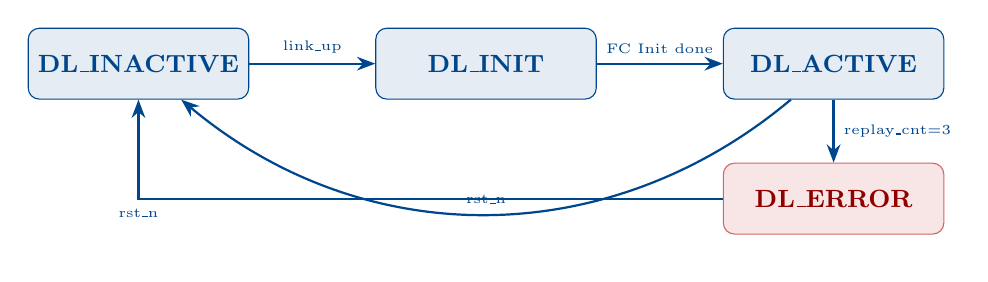
\begin{tikzpicture}[
  state/.style={draw=scblue,fill=scblue!10,rounded corners=4pt,
                minimum width=28mm,minimum height=9mm,align=center,
                font=\small\bfseries,text=scblue},
  err/.style={state,fill=scred!10,draw=scred!60,text=scred!80!black},
  arr/.style={-Stealth,thick,scblue},
  >=Stealth,node distance=8mm and 16mm
]
\definecolor{scred}{RGB}{180,0,0}
\node[state] (inactive) {DL\_INACTIVE};
\node[state,right=of inactive] (init) {DL\_INIT};
\node[state,right=of init] (active) {DL\_ACTIVE};
\node[err,below=of active] (error) {DL\_ERROR};

\draw[arr] (inactive) -- node[above,font=\tiny]{link\_up} (init);
\draw[arr] (init) -- node[above,font=\tiny]{FC Init done} (active);
\draw[arr] (active.south) -- node[right,font=\tiny]{replay\_cnt=3} (error.north);
\draw[arr] (error.west) -| node[below,font=\tiny]{rst\_n} (inactive.south);
\draw[arr] (active) to[bend left=40] node[above,font=\tiny]{rst\_n} (inactive);
\end{tikzpicture}
\end{center}

\begin{description}[leftmargin=3.5cm, style=nextline]
  \item[DL\_INACTIVE] LTSSM not yet in L0; DLL TX holds off all packet emission.
  \item[DL\_INIT] LTSSM has reached L0; FC Init DLLP exchange in progress.
  \item[DL\_ACTIVE] FC Init complete; \texttt{dll\_link\_active} asserted; normal TLP and DLLP traffic allowed.
  \item[DL\_ERROR] Unrecoverable DLL error (replay overflow or fatal DLCRC error); \texttt{dll\_error} asserted; requires link reset.
\end{description}

\subsection{Flow Control}

Credit-based flow control per PCIe~7.0 \S2.11:
\begin{itemize}[noitemsep]
  \item Three categories: Posted (P), Non-Posted (NP), Completion (CPL)
  \item Header credits (12-bit) and Data credits (20-bit, units of 4\,DW)
  \item Infinite credit encoding: all-ones (12'hFFF / 20'hFFFFF)
  \item FC Init handshake: INIT1 then INIT2 for each category
  \item Credit return: received FC Update DLLPs advance remote credit counters in \texttt{pcie\_flow\_ctrl.sv}
  \item Threshold-based FC Update: fires when consumed credits exceed 25\% of total allocated
  \item FC Update type selection: round-robin P $\to$ NP $\to$ CPL per update cycle
  \item Periodic FC Update: timer-driven at 200\,000-cycle intervals (backup)
\end{itemize}

\subsection{TLP Types Supported}

\begin{tabular}{llllp{5cm}}
  \toprule
  \theadcell{TLP Type} & \theadcell{Code} & \theadcell{fmt[2:0]} & \theadcell{Dir} & \theadcell{Description} \\
  \midrule
  Memory Read 32-bit    & MRd32    & 3'b000 & TX/RX & No data, 3DW header, 32-bit addr \\
  Memory Read 64-bit    & MRd64    & 3'b001 & TX/RX & No data, 4DW header, 64-bit addr \\
  Memory Write 32-bit   & MWr32    & 3'b010 & TX/RX & With data, 3DW header \\
  Memory Write 64-bit   & MWr64    & 3'b011 & TX/RX & With data, 4DW header \\
  IO Read               & IORd     & 3'b000 & RX    & 3DW header, IO address space \\
  IO Write              & IOWr     & 3'b010 & RX    & 3DW header + data \\
  Config Read Type 0    & CfgRd0   & 3'b000 & RX    & Local function configuration \\
  Config Read Type 1    & CfgRd1   & 3'b000 & RX    & Forwarded (Root/Switch only) \\
  Config Write Type 0   & CfgWr0   & 3'b010 & RX    & Local function configuration \\
  Config Write Type 1   & CfgWr1   & 3'b010 & RX    & Forwarded (Root/Switch only) \\
  Completion            & Cpl      & 3'b000 & TX/RX & Status only; no data payload \\
  Completion + Data     & CplD     & 3'b010 & TX/RX & Carries read response data \\
  Message               & Msg      & 3'b001 & TX/RX & 4DW header, no data \\
  Message + Data        & MsgD     & 3'b011 & TX/RX & 4DW header + data \\
  AtomicOp Request      & AtomicOpReq & 3'b011 & RX & AtomicOp with data (FetchAdd/Swap/CAS) \\
  AtomicOp Completion   & AtomicOpCpl & 3'b010 & TX & Carries original value \\
  \bottomrule
\end{tabular}

\vspace{2mm}
\noindent\textbf{fmt[2:0] field encoding:} bit[2] = has\_data payload, bit[1] = 4DW address (64-bit), bit[0] = TLP prefix present.

\vspace{2mm}
\noindent\textbf{Traffic Class (TC[2:0]) and Virtual Channel mapping:}
TC[2:0] is encoded in TLP DW0 bits [22:20]. By default, all TCs map to VC0
(single virtual channel). The TLP RX router does not filter on TC.
VC/TC mapping registers are in the PCIe Extended Capability (offset 0x14C--0x17C),
planned for v0.3.0 multi-VC support.

\subsection{Link Equalization (Gen3+)}
\label{subsec:equalization}

PCIe Gen3 and above require link equalization to compensate for insertion loss,
crosstalk, and reflections at high data rates. The LTSSM implements a 4-phase
equalization process in \texttt{pcie\_ltssm.sv} using per-phase timers
(\texttt{EQ\_PHASE1\_TIMEOUT}, \texttt{EQ\_PHASE2\_TIMEOUT},
\texttt{EQ\_PHASE3\_TIMEOUT} from \texttt{pcie\_pkg.sv}).

\begin{table}[h!]
\centering
\begin{tabular}{p{1.2cm}p{3cm}p{3.5cm}p{7cm}}
  \toprule
  \theadcell{Phase} & \theadcell{Name} & \theadcell{Duration (Timeout)} & \theadcell{Description} \\
  \midrule
  Phase 0 & Preset Application & N/A (instantaneous) & Both sides apply preset TX coefficients (pre-cursor, cursor, post-cursor) from the RECOVERY\_EQ state. No timer; proceeds immediately to Phase 1. \\
  Phase 1 & DS Requests US     & \texttt{EQ\_PHASE1\_TIMEOUT} = 2\,ms & Downstream component transmits TS2 ordered sets with equalization request; requests upstream to evaluate downstream coefficients. Timer guards against unresponsive link partner. \\
  Phase 2 & US Evaluates       & \texttt{EQ\_PHASE2\_TIMEOUT} = 2\,ms & Upstream component evaluates received signal quality and requests preferred downstream TX coefficients via TS2 feedback. Both sides may iterate. \\
  Phase 3 & Verification       & \texttt{EQ\_PHASE3\_TIMEOUT} = 50\,$\mu$s & Both sides confirm final coefficients are acceptable and signal equalization complete. Link proceeds to CONFIG or RECOVERY\_IDLE on success. \\
  \bottomrule
\end{tabular}
\caption{PCIe Gen3+ Link Equalization Phases (implemented in RECOVERY\_EQUALIZATION state)}
\end{table}

The current equalization phase is reflected on the \texttt{eq\_phase[2:0]} output
port and in \texttt{ltssm\_status[4:2]}. Phase timeout causes a fallback to
RECOVERY\_RCVRLOCK for re-attempt.

% =============================================================================
\section{Configuration Space Register Map}
% =============================================================================

\subsection{Standard Capability Registers}

\begin{longtable}{p{2.5cm}p{4.5cm}p{1.5cm}p{5.5cm}}
  \toprule
  \theadcell{Offset} & \theadcell{Register Name} & \theadcell{Access} & \theadcell{Description} \\
  \midrule
  \endhead
  \multicolumn{4}{r}{\small\itshape continued on next page} \\
  \endfoot
  \endlastfoot
  0x000        & Vendor/Device ID   & RO    & \{DEVICE\_ID[15:0], VENDOR\_ID[15:0]\} \\
  0x004        & Command/Status     & RW/RO & PCI command (I/O space en, bus master en, mem space en, SERR en) \\
  0x008        & Revision/Class     & RO    & \{CLASS\_CODE[23:0], REVISION\_ID[7:0]\} \\
  0x00C        & Cache Line / Lat.  & RW/RO & Cache line size [7:0], latency timer [15:8], header type [23:16] \\
  0x010--0x024 & BAR0--BAR5         & RW    & BAR0--BAR1 = 64-bit prefetchable; BAR2--BAR5 = 32-bit \\
  0x02C        & Subsystem IDs      & RO    & \{SubsysDevice[31:16], SubsysVendor[15:0]\} \\
  0x034        & Cap Pointer        & RO    & 0x40 (points to PCIe Capability) \\
  0x03C        & Interrupt Line/Pin & RW/RO & Interrupt line [7:0]; pin = INTA (0x01) \\
  \midrule
  \multicolumn{4}{l}{\textit{PCIe Express Capability (starting at 0x040)}} \\
  \midrule
  0x040        & PCIe Cap Register  & RO    & [3:0] = Capability version (0x2); [7:4] = Device/Port type (0x0 = EP); [8] = Slot implemented; [13:9] = IRQ number \\
  0x044        & Device Capabilities & RO   & [2:0] = Max payload size supported (010 = 512\,B); [4:3] = Phantom functions (00); [5] = Extended tag field (1 = 10-bit tags); [8:6] = EP L0s acceptable latency; [11:9] = EP L1 acceptable latency \\
  0x048        & Device Control     & RW    & [0] = Correctable error reporting en; [1] = Non-fatal error reporting en; [2] = Fatal error reporting en; [3] = UR reporting en; [4] = Enable relaxed ordering; [7:5] = Max payload size; [8] = Extended tag field en; [11] = Enable no-snoop; [14:12] = Max read request size; [15] = BCRE/initiate FLR \\
  0x04A        & Device Status      & RW1C  & [0] = Corr. error detected; [1] = Non-fatal error detected; [2] = Fatal error detected; [3] = UR detected; [4] = AUX power detected; [5] = Transactions pending \\
  0x04C        & Link Capabilities  & RO    & [3:0] = Max link speed (0111 = Gen7); [9:4] = Max link width (010000 = $\times$16); [11:10] = ASPM support (11 = L0s+L1); [14:12] = L0s exit latency; [17:15] = L1 exit latency; [18] = Clock PM; [19] = Surprise down error; [20] = Data link active; [21] = Link BW notification cap \\
  0x050        & Link Control       & RW    & [1:0] = ASPM control; [3] = RCB (read completion boundary); [4] = Link disable; [5] = Retrain link; [6] = Common clock config; [7] = Extended sync; [8] = Clock PM en; [9] = HW autonomous width disable; [10] = Link BW management status en; [11] = Link autonomous BW status en \\
  0x052        & Link Status        & RO    & [3:0] = Current link speed; [9:4] = Negotiated link width; [11] = Link training; [12] = Slot clock config; [13] = Data link active; [14] = Link BW management status; [15] = Link autonomous BW status \\
  \midrule
  \multicolumn{4}{l}{\textit{Slot Capability Registers (0x058, if slot implemented)}} \\
  \midrule
  0x058        & Slot Capabilities  & RO    & [0] = Attention button; [1] = Power controller; [2] = MRL sensor; [3] = Attention indicator; [4] = Power indicator; [5] = Hot-plug surprise; [6] = Hot-plug capable; [14:7] = Slot power limit value; [16:15] = Slot power limit scale; [17] = EMI lock; [24] = Physical slot number[12:0] \\
  \midrule
  \multicolumn{4}{l}{\textit{Power Management Capability (at 0x080)}} \\
  \midrule
  0x080--0x084 & PM Capability      & RW/RO & PME support D0/D3hot/D3cold; power state control; PME status/enable \\
  \midrule
  \multicolumn{4}{l}{\textit{MSI Capability (at 0x090)}} \\
  \midrule
  0x090--0x09C & MSI Capability     & RW    & MSI Enable, 64-bit addr, multiple msg en/cap (5 bits = 32 vectors) \\
  \midrule
  \multicolumn{4}{l}{\textit{MSI-X Capability (at 0x0A0)}} \\
  \midrule
  0x0A0--0x0A8 & MSI-X Capability   & RW    & MSI-X Enable, function mask; table size = 2047 (2048 vectors); table BIR and offset; PBA BIR and offset \\
  \bottomrule
\end{longtable}

\subsection{AER Extended Capability Registers (Base: 0x100)}

The Advanced Error Reporting (AER) capability is an Extended Capability structure
located at offset 0x100 in the 4\,KB extended configuration space.

\begin{longtable}{p{2.5cm}p{4.5cm}p{1.5cm}p{5.5cm}}
  \toprule
  \theadcell{Offset} & \theadcell{Register Name} & \theadcell{Access} & \theadcell{Description} \\
  \midrule
  \endhead
  \multicolumn{4}{r}{\small\itshape continued on next page} \\
  \endfoot
  \endlastfoot
  0x100 & AER Enhanced Capability Header & RO & [15:0] = AER Cap ID (0x0001); [19:16] = Cap version (0x2); [31:20] = Next cap offset (0x000 = last) \\
  0x104 & Uncorrectable Error Status     & RW1C & Bit-mapped uncorrectable errors: [4]=DL Proto Error, [12]=Poisoned TLP Rcvd, [13]=FC Protocol Error, [14]=Completion Timeout, [15]=Completer Abort, [16]=Unexpected Cpl, [17]=Receiver Overflow, [18]=Malformed TLP, [19]=ECRC Error, [20]=UR, [21]=ACS Violation \\
  0x108 & Uncorrectable Error Mask       & RW   & Per-bit enable mask; 1 = masked (not reported). Default: all zero (all reported) \\
  0x10C & Uncorrectable Error Severity   & RW   & Per-bit severity: 0 = Non-fatal, 1 = Fatal. Default: DL Proto Error = Fatal; others = Non-fatal \\
  0x110 & Correctable Error Status       & RW1C & [0]=Receiver Error, [6]=Bad TLP, [7]=Bad DLLP, [8]=Replay Num Rollover, [12]=Replay Timer Timeout, [13]=Advisory Non-Fatal Error, [14]=Corrected Internal Error \\
  0x114 & Correctable Error Mask         & RW   & Per-bit mask; 1 = masked. Default: Advisory Non-Fatal Error masked \\
  0x118 & Advanced Error Cap and Control & RW   & [4:0] = First error pointer; [5] = ECRC generation capable; [6] = ECRC generation enable; [7] = ECRC check capable; [8] = ECRC check enable; [9] = Multiple header recording; [10] = TLP prefix log present \\
  0x11C & Header Log Register [0]        & RO   & First DW of TLP header that caused the first uncorrectable error \\
  0x120 & Header Log Register [1]        & RO   & Second DW of captured TLP header \\
  0x124 & Header Log Register [2]        & RO   & Third DW of captured TLP header \\
  0x128 & Header Log Register [3]        & RO   & Fourth DW of captured TLP header (0 for 3DW TLPs) \\
  \bottomrule
\end{longtable}

% =============================================================================
\section{Clock and Reset Architecture}
% =============================================================================

\subsection{Clock Domains}

\begin{tabular}{p{2.5cm}p{3cm}p{3cm}p{5cm}}
  \toprule
  \theadcell{Domain} & \theadcell{Clock Port} & \theadcell{Typical Freq.} & \theadcell{Contents} \\
  \midrule
  PD\_CORE & \texttt{core\_clk} & 250\,MHz & LTSSM, DLL, FC, TL, AXI bridge, DMA, completion timeout \\
  PD\_PIPE & \texttt{pipe\_clk} & 500\,MHz (Gen7) & PIPE adapter gearbox \\
  PD\_AUX  & \texttt{aux\_clk}  & 32\,kHz (real) or 100\,MHz (sim) & PM controller, retention registers \\
  \bottomrule
\end{tabular}

\subsection{CDC Crossings Summary}

\begin{tabular}{p{1.5cm}p{3cm}p{3cm}p{6cm}}
  \toprule
  \theadcell{ID} & \theadcell{Crossing} & \theadcell{Mitigation} & \theadcell{Signals} \\
  \midrule
  CDC-001 & core $\to$ pipe  & \texttt{pcie\_sync2} per-bit & \texttt{pipe\_rate}, \texttt{pipe\_width}, \texttt{pipe\_power\_down} \\
  CDC-002 & pipe $\to$ core  & \texttt{pcie\_async\_fifo} & RX data bus \\
  CDC-003 & core $\to$ aux   & \texttt{pcie\_sync2} per-bit & PM control signals \\
  CDC-004 & aux $\to$ core   & \texttt{pcie\_sync\_pulse}   & PME wake pulse \\
  CDC-005 & async $\to$ *    & \texttt{pcie\_rst\_sync}    & \texttt{core\_rst\_n} deassertion \\
  \bottomrule
\end{tabular}

\subsection{Reset Sequence}

\begin{enumerate}[noitemsep]
  \item Assert \texttt{core\_rst\_n} low (active). All registers initialize to reset state.
  \item Bring up \texttt{core\_clk} and \texttt{aux\_clk}; initialize PHY.
  \item When PHY asserts \texttt{pipe\_clk} valid, bring up \texttt{pipe\_clk}.
  \item Hold all clocks stable for $\geq 100$\,ns.
  \item Deassert \texttt{core\_rst\_n} high; synchronized internally by \texttt{pcie\_rst\_sync}.
  \item LTSSM starts from \texttt{DETECT\_QUIET} automatically.
\end{enumerate}

% =============================================================================
\section{Power Management}
% =============================================================================

\subsection{Power States}

\begin{tabular}{p{2cm}p{3.5cm}p{2.5cm}p{6cm}}
  \toprule
  \theadcell{State} & \theadcell{Entry} & \theadcell{Exit} & \theadcell{Description} \\
  \midrule
  L0   & Power-on / wakeup & N/A    & Full operation; \texttt{link\_up} asserted \\
  L0s  & EIOS receipt (auto, 64+ idle beats) & Any TLP / SKP OS & Low-latency autonomous power save; driven by \texttt{dllp\_pm\_req\_l1=0}; L0s exit timeout from \texttt{pcie\_pkg}: \texttt{L0S\_EXIT\_TIMEOUT} \\
  L1   & SW request + PM DLLP handshake (\texttt{dllp\_pm\_req\_l1/dllp\_pm\_ack}) & PME / SW & PM\_Enter\_L1 / PM\_Req\_Ack exchange; PIPE powered down to P1; L1 exit timeout: \texttt{L1\_EXIT\_TIMEOUT} \\
  L2   & SW via PM register & PME / CLKREQ & Deep sleep; core may power down; aux retained; requires full link re-training on wake \\
  \bottomrule
\end{tabular}

\subsection{UPF Power Domains}

Three power domains defined in \texttt{rtl/pcie\_controller\_top.upf}:

\begin{itemize}[noitemsep]
  \item \textbf{PD\_CORE} (VDD\_CORE 1.0\,V) --- always-on during L0/L0s/L1; may power down in L2
  \item \textbf{PD\_PIPE} (VDD\_PIPE 1.0\,V) --- may power down in L1 and L2
  \item \textbf{PD\_AUX}  (VDD\_AUX 0.9\,V) --- always retained; holds PM FSM state
\end{itemize}

% =============================================================================
\section{Verification Collateral}
% =============================================================================

\subsection{Directed Testbench (iverilog)}

\begin{tabular}{lp{10cm}}
  \toprule
  \theadcell{Test} & \theadcell{Coverage} \\
  \midrule
  1. Link Training    & LTSSM: DETECT $\to$ POLLING $\to$ CONFIG $\to$ L0 \\
  2. Negotiated Params & Gen and width within valid range after link-up \\
  3. Config Space Init & Link stable after config-space initialization \\
  4. MPS/MRRS Fields  & Max Payload and Max Read Request Size \\
  5. AXI Write        & AXI4 write generates MWr TLP on PIPE TX \\
  6. AXI Read         & AXI4 read generates MRd TLP; CplD returns \\
  7. DMA H2D          & MRd64 chunked; completions assembled \\
  8. DMA D2H          & Local read; MWr64 issued to host \\
  9. MSI Interrupt    & INTx assertion triggers MSI IRQ \\
  10. AER Error       & No spurious errors in steady-state L0 \\
  \bottomrule
\end{tabular}

\subsection{UVM Testbench}

\begin{tabular}{lp{10cm}}
  \toprule
  \theadcell{Component} & \theadcell{Description} \\
  \midrule
  \texttt{pcie\_axi\_agent}        & Sequencer, driver, monitor on AXI subordinate interface \\
  \texttt{pcie\_pipe\_agent}       & PIPE-level driver (RX stimuli), monitor (TX capture) \\
  \texttt{pcie\_scoreboard}        & AXI response check; error count \\
  \texttt{pcie\_coverage}          & AXI direction $\times$ response cross coverage \\
  \texttt{pcie\_ltssm\_cov}        & 28-state, transition, and Gen$\times$width coverage \\
  \texttt{pcie\_error\_regression\_test} & Bad LCRC, NAK, replay timeout, malformed TLP, poisoned TLP, cpl timeout, FC exhaust \\
  \bottomrule
\end{tabular}

\subsection{SVA Assertion Modules}

\begin{tabular}{lp{9.5cm}}
  \toprule
  \theadcell{Module} & \theadcell{Properties} \\
  \midrule
  \texttt{pcie\_ltssm\_assertions}    & 12 assert + 12 cover: state validity, link\_up/L0 consistency, power control, liveness, EQ phase sequence \\
  \texttt{pcie\_dll\_assertions}      & 15 assert + 9 cover: backpressure, DLLP type, burst integrity, replay\_count $\le$ 3, dll\_active consistency, FC/PM DLLP type assertions, DLCRC error isolation \\
  \texttt{pcie\_fc\_assertions}       & 13 assert + 8 cover: credit underflow/overflow, liveness, credit-return from FC Update DLLPs, FC update type round-robin check \\
  \texttt{pcie\_tlp\_assertions}      & 11 assert + 8 cover: AXI protocol, TLP framing, DMA exclusion, error signal exclusion \\
  \texttt{pcie\_delivery\_assertions} & 20 assert + 10 cover: TLP delivery X-check, AXI ordering, DMA channel exclusion, backpressure stall, error-flag exclusion, FC liveness, DLLP activity in DL\_ACTIVE \\
  \bottomrule
\end{tabular}

% =============================================================================
\section{Delivery Checklist}
% =============================================================================

\begin{tabular}{lll}
  \toprule
  \theadcell{Item} & \theadcell{File(s)} & \theadcell{Status} \\
  \midrule
  RTL source (16 modules)          & \texttt{rtl/*.sv}                        & \checkmark \\
  Package with types and functions & \texttt{rtl/pcie\_pkg.sv}                & \checkmark \\
  Directed testbench               & \texttt{tb/*.sv}                         & \checkmark \\
  UVM testbench (8 components)     & \texttt{uvm\_tb/*.sv}                    & \checkmark \\
  SVA assertion suites (5 modules) & \texttt{sva/*.sv}                        & \checkmark \\
  Formal FPV setups (3 targets)    & \texttt{formal/*.sby}                    & \checkmark \\
  Synthesis script (DC)            & \texttt{scripts/synth\_dc.tcl}           & \checkmark \\
  SDC timing constraints           & \texttt{constraints/*.sdc}               & \checkmark \\
  UPF power intent                 & \texttt{rtl/*.upf}                       & \checkmark \\
  IP-XACT descriptor               & \texttt{ip\_xact/*.xml}                  & \checkmark \\
  Coverage merge script            & \texttt{scripts/coverage\_merge.sh}      & \checkmark \\
  Release package script           & \texttt{scripts/release\_package.sh}     & \checkmark \\
  CDC waiver log                   & \texttt{lint/cdc\_waivers.md}            & \checkmark \\
  Integration guide                & \texttt{docs/integration\_guide.md}      & \checkmark \\
  Compliance matrix                & \texttt{docs/compliance\_matrix.md}      & \checkmark \\
  Specification                    & \texttt{docs/latex/pcie\_specification.pdf} & \checkmark \\
  Project report                   & \texttt{docs/latex/pcie\_project\_report.pdf} & \checkmark \\
  \bottomrule
\end{tabular}

\vspace{4mm}
\noindent\textbf{Remaining for production signoff:} FLIT-mode framing (v0.3.0), TLP ordering
enforcement, UVM regression with commercial simulator coverage archive, CDC tool
report review, synthesis timing closure at corner.

% =============================================================================
\section*{Acceptance Criteria}
% =============================================================================
\addcontentsline{toc}{section}{Acceptance Criteria}

\begin{enumerate}[noitemsep]
  \item RTL compiles from a clean checkout using \texttt{filelists/rtl.f}.
  \item \texttt{make sim} (iverilog) passes all 10 directed tests: 10/10 PASS.
  \item UVM smoke and error regression tests complete without UVM\_FATAL or UVM\_ERROR.
  \item Lint is either clean or all warnings are documented in \texttt{lint/waivers.vlt}.
  \item All 5 CDC crossings are mitigated per \texttt{lint/cdc\_waivers.md}.
  \item Formal FPV (\texttt{formal/*.sby}) reports no assertion failures.
  \item DLCRC-16 (poly 0x8005) is computed and verified on all DLLPs; \texttt{dllp\_err} fires on mismatch.
  \item DLL replay count does not exceed REPLAY\_COUNT\_MAX=3 before \texttt{dll\_error} is asserted.
  \item Equalization completes within per-phase timeouts (Phase1/2: 2\,ms, Phase3: 50\,$\mu$s) for Gen3+ links.
  \item All known issues are documented in \texttt{docs/known\_issues.md}.
  \item Signoff checklist (\texttt{docs/signoff\_checklist.md}) is fully reviewed before release.
\end{enumerate}

\end{document}
